\chapter{Introduction}
\label{cha:Introduction} % Ein Label ist optional, ermoeglicht aber die Referenzierung
\textbf{\color{red}THIS IS NOT FINAL}

In this chapter we will explore the motivation and goals of this seminar thesis, as well its structure.
In order to do this, we will explain the motivation behind the topic as well as the research questions that we aim to answer in section \ref{sec:motivation-goals} \nameref{sec:motivation-goals}.
Afterwards we will then explain the thesis's structure and contents in section \ref{sec:structure} \nameref{sec:structure}.

\section{Motivation and Goals}
\label{sec:motivation-goals}
This chapter delves into the motivation behind this thesis and furthermore defines research questions, which we aim to answer in the subsequent chapters.

% Introduction: lots of data -> cant save it all -> need a way to deal with it
% Examples of when it is applied
% How does it work, are there alternatives? yes -> batch processing (Maybe briefly explain)
The advancements in technology of the past decades has lead to enormous data creation. Technology has become ubiquitous, 
with the evolution of cell phones to smartphones, the digitilization of industrial processes, Industry 4.0
and the increasing amount of ``smart`` devices, causing creation of information to grow exponentially.
It is estimated that the \gls{datasphere} will reach the size of 175 zettabytes by 2025, as shown in figure \ref{fig:growth_datasphere}.
% Graph estimating the growth of the global datasphere (by IDC)
\begin{figure}[ht]
\centering
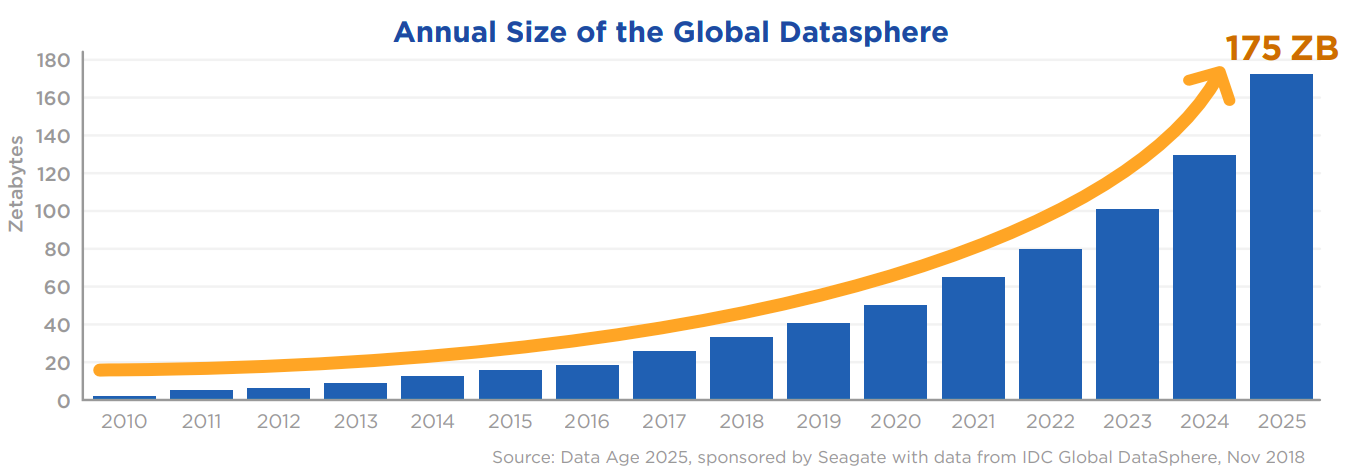
\includegraphics[width=1.0\textwidth]{Bilder/size_global_datasphere.png}
\caption{The Growth of the Global Datasphere \cite[p.6]{idc-seagate-data}}
\label{fig:growth_datasphere}
\end{figure}`

% Maybe a source here?
Data has become an important factor in decision making and optimization in virtually every industry, especially in finances. \textbf{TODO: Wieso?}
The financial market is dominated by data driven decisions, with emphasis on data processing in a (near) real-time fashion.
However, real-time data is becoming of importance in multiple sectors; the International Data Corporation estimates that real-time data will be 
responsible for a share of 30 percent of the total global datasphere by 2025, as shown in figure \ref{fig:growth_realtime_data}.
% Graph showing the growing share of real-time data as part of global datasphere
\begin{figure}[h]
\centering
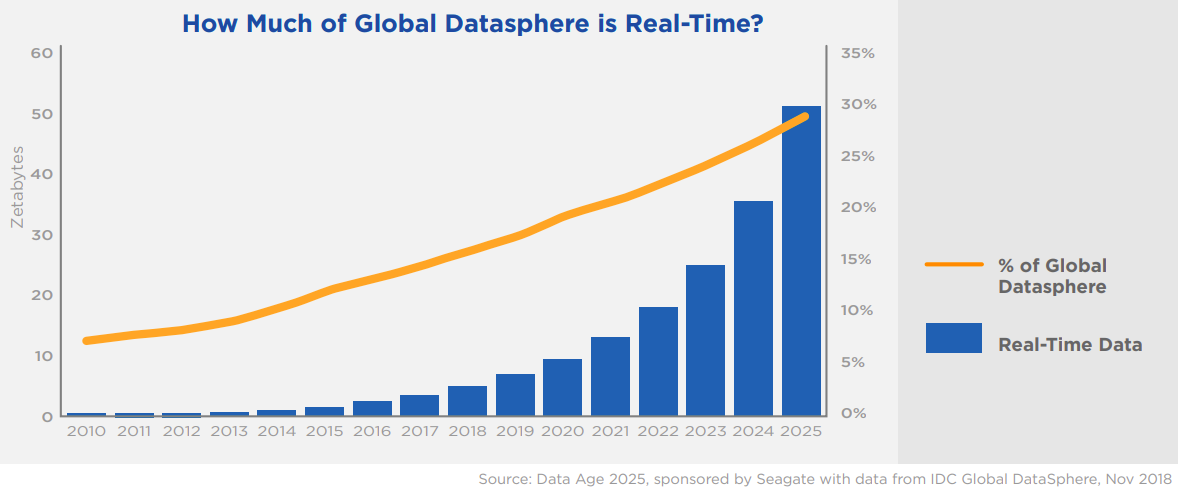
\includegraphics[width=1.0\textwidth]{Bilder/realtime_data.png}
\caption{The growth of real-time data as part of the Global Datasphere \cite[p.13]{idc-seagate-data}}
\label{fig:growth_realtime_data}
\end{figure}

A global study led by IBM in 2012 has shown that 71 percent of the firms in the financial market use information (including big data)
in order to achieve an advantage over their competitors, compared to 36 percent, which IBM has found in an earlier study conducted in 2010. \cite[p.1]{ibm-financial}

As it is no longer feasible to save all the data before then analyzing it (in batches), due to computational cost and lack of storage capacity, 
a new approach was designed in order to handle data in a (near) real-time fashion, Stream Processing Systems (SPS).

However the rate in which data is being streamed fluctuates, so one comes to the logical conclusion that SPSs should adapt to the velocity and volume of the stream.
Besides the stream, the computing environment might also fluctuate, e.g. a resource failing in a distributed computing environment, 
and as such the system has to adapt. There are many different techniques of adaptation such a system might utilize, 
which can impact both the stream as well as the SPS. We will elaborate on this in \ref{sub:sps} \nameref{sub:sps}.


\textbf{TODO: Why self adaptivity is needed? Research different kinds of adaptation (e.g. load shedding, elastric allocation of resources), look at cui's paper, add concrete examples
Structure:
Why stream processing? -> Why adaptive?}

RESEARCH QUESTIONS:

1. What is Stream Processing?

2. What are possible techniques for adapatation in stream processing?

3. Why is self-adaptivity needed in Stream processing?

4. What are current approaches in self-adaptive stream processing?


\section{Structure}
\label{sec:structure}
Explain Structure and contents of chapters here